% Generated by scripts/build_rq2_site_analysis.py — do not edit by hand.
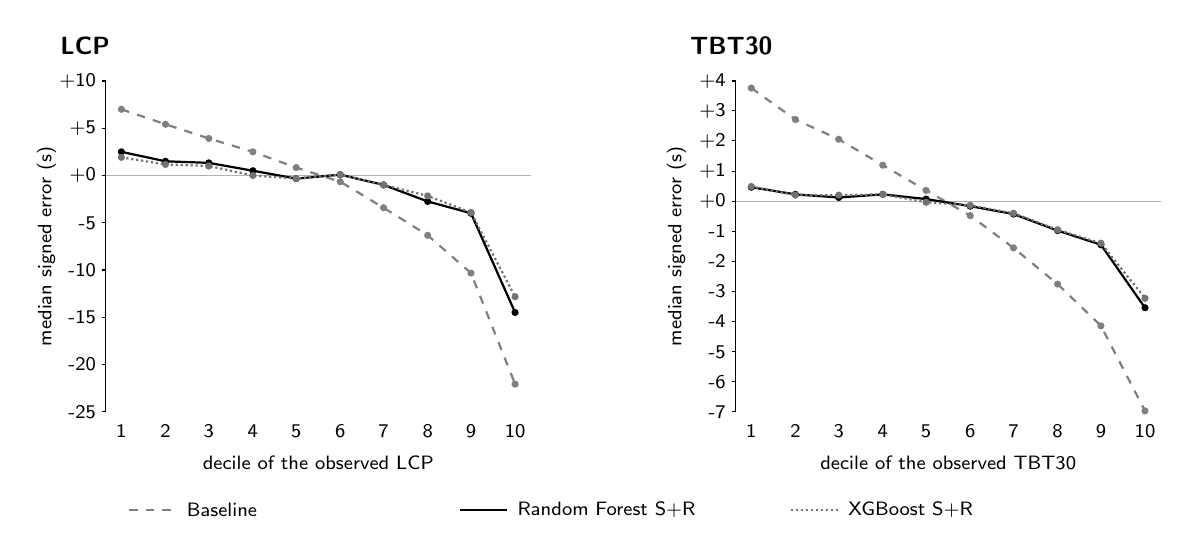
\begin{tikzpicture}[font=\sffamily\scriptsize]
\node[font=\sffamily\bfseries\small, anchor=west] at (0.0,4.65) {LCP};
\draw (0.70,0) -- (0.70,4.2);
\draw (0.65,0.00) -- (0.70,0.00) node[left] {-25};
\draw (0.65,0.60) -- (0.70,0.60) node[left] {-20};
\draw (0.65,1.20) -- (0.70,1.20) node[left] {-15};
\draw (0.65,1.80) -- (0.70,1.80) node[left] {-10};
\draw (0.65,2.40) -- (0.70,2.40) node[left] {-5};
\draw (0.65,3.00) -- (0.70,3.00) node[left] {+0};
\draw (0.65,3.60) -- (0.70,3.60) node[left] {+5};
\draw (0.65,4.20) -- (0.70,4.20) node[left] {+10};
\draw[gray!60] (0.70,3.00) -- (6.10,3.00);
\node at (0.90,-0.25) {1};
\node at (1.46,-0.25) {2};
\node at (2.01,-0.25) {3};
\node at (2.57,-0.25) {4};
\node at (3.12,-0.25) {5};
\node at (3.68,-0.25) {6};
\node at (4.23,-0.25) {7};
\node at (4.79,-0.25) {8};
\node at (5.34,-0.25) {9};
\node at (5.90,-0.25) {10};
\node at (3.40,-0.65) {decile of the observed LCP};
\node[rotate=90] at (-0.05,2.10) {median signed error (s)};
\draw[gray, dashed, thick] (0.90,3.84) -- (1.46,3.65) -- (2.01,3.47) -- (2.57,3.30) -- (3.12,3.10) -- (3.68,2.92) -- (4.23,2.59) -- (4.79,2.24) -- (5.34,1.76) -- (5.90,0.35);
\fill[gray] (0.90,3.84) circle (1.3pt);
\fill[gray] (1.46,3.65) circle (1.3pt);
\fill[gray] (2.01,3.47) circle (1.3pt);
\fill[gray] (2.57,3.30) circle (1.3pt);
\fill[gray] (3.12,3.10) circle (1.3pt);
\fill[gray] (3.68,2.92) circle (1.3pt);
\fill[gray] (4.23,2.59) circle (1.3pt);
\fill[gray] (4.79,2.24) circle (1.3pt);
\fill[gray] (5.34,1.76) circle (1.3pt);
\fill[gray] (5.90,0.35) circle (1.3pt);
\draw[black, solid, thick] (0.90,3.30) -- (1.46,3.18) -- (2.01,3.16) -- (2.57,3.06) -- (3.12,2.96) -- (3.68,3.01) -- (4.23,2.88) -- (4.79,2.67) -- (5.34,2.52) -- (5.90,1.26);
\fill[black] (0.90,3.30) circle (1.3pt);
\fill[black] (1.46,3.18) circle (1.3pt);
\fill[black] (2.01,3.16) circle (1.3pt);
\fill[black] (2.57,3.06) circle (1.3pt);
\fill[black] (3.12,2.96) circle (1.3pt);
\fill[black] (3.68,3.01) circle (1.3pt);
\fill[black] (4.23,2.88) circle (1.3pt);
\fill[black] (4.79,2.67) circle (1.3pt);
\fill[black] (5.34,2.52) circle (1.3pt);
\fill[black] (5.90,1.26) circle (1.3pt);
\draw[black!55, densely dotted, thick] (0.90,3.23) -- (1.46,3.14) -- (2.01,3.12) -- (2.57,3.00) -- (3.12,2.96) -- (3.68,3.01) -- (4.23,2.88) -- (4.79,2.74) -- (5.34,2.53) -- (5.90,1.46);
\fill[black!55] (0.90,3.23) circle (1.3pt);
\fill[black!55] (1.46,3.14) circle (1.3pt);
\fill[black!55] (2.01,3.12) circle (1.3pt);
\fill[black!55] (2.57,3.00) circle (1.3pt);
\fill[black!55] (3.12,2.96) circle (1.3pt);
\fill[black!55] (3.68,3.01) circle (1.3pt);
\fill[black!55] (4.23,2.88) circle (1.3pt);
\fill[black!55] (4.79,2.74) circle (1.3pt);
\fill[black!55] (5.34,2.53) circle (1.3pt);
\fill[black!55] (5.90,1.46) circle (1.3pt);
\node[font=\sffamily\bfseries\small, anchor=west] at (8.0,4.65) {TBT30};
\draw (8.70,0) -- (8.70,4.2);
\draw (8.65,0.00) -- (8.70,0.00) node[left] {-7};
\draw (8.65,0.38) -- (8.70,0.38) node[left] {-6};
\draw (8.65,0.76) -- (8.70,0.76) node[left] {-5};
\draw (8.65,1.15) -- (8.70,1.15) node[left] {-4};
\draw (8.65,1.53) -- (8.70,1.53) node[left] {-3};
\draw (8.65,1.91) -- (8.70,1.91) node[left] {-2};
\draw (8.65,2.29) -- (8.70,2.29) node[left] {-1};
\draw (8.65,2.67) -- (8.70,2.67) node[left] {+0};
\draw (8.65,3.05) -- (8.70,3.05) node[left] {+1};
\draw (8.65,3.44) -- (8.70,3.44) node[left] {+2};
\draw (8.65,3.82) -- (8.70,3.82) node[left] {+3};
\draw (8.65,4.20) -- (8.70,4.20) node[left] {+4};
\draw[gray!60] (8.70,2.67) -- (14.10,2.67);
\node at (8.90,-0.25) {1};
\node at (9.46,-0.25) {2};
\node at (10.01,-0.25) {3};
\node at (10.57,-0.25) {4};
\node at (11.12,-0.25) {5};
\node at (11.68,-0.25) {6};
\node at (12.23,-0.25) {7};
\node at (12.79,-0.25) {8};
\node at (13.34,-0.25) {9};
\node at (13.90,-0.25) {10};
\node at (11.40,-0.65) {decile of the observed TBT30};
\node[rotate=90] at (7.95,2.10) {median signed error (s)};
\draw[gray, dashed, thick] (8.90,4.11) -- (9.46,3.71) -- (10.01,3.46) -- (10.57,3.13) -- (11.12,2.81) -- (11.68,2.49) -- (12.23,2.08) -- (12.79,1.62) -- (13.34,1.09) -- (13.90,0.01);
\fill[gray] (8.90,4.11) circle (1.3pt);
\fill[gray] (9.46,3.71) circle (1.3pt);
\fill[gray] (10.01,3.46) circle (1.3pt);
\fill[gray] (10.57,3.13) circle (1.3pt);
\fill[gray] (11.12,2.81) circle (1.3pt);
\fill[gray] (11.68,2.49) circle (1.3pt);
\fill[gray] (12.23,2.08) circle (1.3pt);
\fill[gray] (12.79,1.62) circle (1.3pt);
\fill[gray] (13.34,1.09) circle (1.3pt);
\fill[gray] (13.90,0.01) circle (1.3pt);
\draw[black, solid, thick] (8.90,2.85) -- (9.46,2.76) -- (10.01,2.72) -- (10.57,2.76) -- (11.12,2.70) -- (11.68,2.61) -- (12.23,2.51) -- (12.79,2.30) -- (13.34,2.12) -- (13.90,1.32);
\fill[black] (8.90,2.85) circle (1.3pt);
\fill[black] (9.46,2.76) circle (1.3pt);
\fill[black] (10.01,2.72) circle (1.3pt);
\fill[black] (10.57,2.76) circle (1.3pt);
\fill[black] (11.12,2.70) circle (1.3pt);
\fill[black] (11.68,2.61) circle (1.3pt);
\fill[black] (12.23,2.51) circle (1.3pt);
\fill[black] (12.79,2.30) circle (1.3pt);
\fill[black] (13.34,2.12) circle (1.3pt);
\fill[black] (13.90,1.32) circle (1.3pt);
\draw[black!55, densely dotted, thick] (8.90,2.86) -- (9.46,2.75) -- (10.01,2.75) -- (10.57,2.76) -- (11.12,2.66) -- (11.68,2.62) -- (12.23,2.52) -- (12.79,2.31) -- (13.34,2.14) -- (13.90,1.44);
\fill[black!55] (8.90,2.86) circle (1.3pt);
\fill[black!55] (9.46,2.75) circle (1.3pt);
\fill[black!55] (10.01,2.75) circle (1.3pt);
\fill[black!55] (10.57,2.76) circle (1.3pt);
\fill[black!55] (11.12,2.66) circle (1.3pt);
\fill[black!55] (11.68,2.62) circle (1.3pt);
\fill[black!55] (12.23,2.52) circle (1.3pt);
\fill[black!55] (12.79,2.31) circle (1.3pt);
\fill[black!55] (13.34,2.14) circle (1.3pt);
\fill[black!55] (13.90,1.44) circle (1.3pt);
\draw[gray, dashed, thick] (1.00,-1.25) -- (1.60,-1.25) node[right, black] {Baseline};
\draw[black, solid, thick] (5.20,-1.25) -- (5.80,-1.25) node[right, black] {Random Forest S+R};
\draw[black!55, densely dotted, thick] (9.40,-1.25) -- (10.00,-1.25) node[right, black] {XGBoost S+R};
\end{tikzpicture}